% !TEX TS-program = xelatex
% !TEX encoding = UTF-8 Unicode
% !Mode:: "TeX:UTF-8"
\documentclass[14pt]{resume}
\usepackage{graphicx}
\usepackage{tabu}
\usepackage{multirow}
\usepackage{multicol}
\usepackage{progressbar}
\usepackage{zh_CN-Adobefonts_external}
\usepackage{linespacing_fix}
\usepackage{cite}

\begin{document}
\pagenumbering{gobble}

\begin{multicols}{4}
    \Large{
        \begin{tabu}{ r }
            \multirow{5}{1in}{
                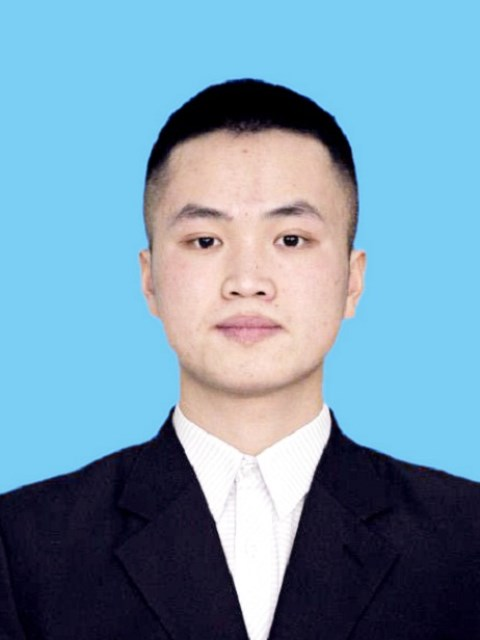
\includegraphics[width=0.88in]{xjl}
            }
        \end{tabu}
    }
    \columnbreak
    \Large{
        \begin{tabu}{ l l }
            & \faBirthdayCake{1996.11.18} \\
            & \phone{(+86)18821657781} \\
            & \email{nwsuafxujianglong@163.com} \\
            %& \homepage[www.zhouweilin.cn]{https://zhouweilin.cn} \\
            & \github[github.com/nwsuafxujianglong]{https://github.com/nwsuafxujianglong} 
        \end{tabu}
    }
    \columnbreak
    \Large{
        \begin{tabu}{ r }
            \multirow{5}{5in}{
                \name{许江龙}
                \basicInfo{
                    \faSmileO{意向职位:软件开发工程师}
                }
            }
        \end{tabu}
    }
\end{multicols}
\vspace{0.5cm}
% 教育背景
\section{\faGraduationCap\  教育背景}
\datedsubsection{\textbf{西北农林科技大学(985、211)\quad}{ 信息工程学院\quad}{ 计算机科学与技术(本科)}}{2015.09 - 2019.06}
\vspace{0.2cm}

% 技能树
\section{\faCogs\ 技能树}

\begin{itemize}
    \item[\faTree] 熟悉Java、C++、C、数据结构与算法
    \item[\faTree] 熟悉Linux操作系统的使用
    \item[\faTree] 熟悉后端框架Spring、Django
    \item[\faTree] 了解git原理及多人协作开发方式
    \item[\faTree] 熟悉python、了解中间件EJB、mySQL数据库
    \item[\faTree] 熟悉计算机网络、操作系统、编译原理、计算机组成原理等基础知识
    \item[\faTree] 熟练使用Google、Stack Overflow、CSDN、Github检索
\end{itemize}
% 项目经历
\section{\faUsers\ 项目经历}

\datedsubsection{\textbf{基于Django的网上预约卖车系统 \hfill}{设计、实现与测试}}{\faCalendar\enskip2018.05 - 07}
\begin{onehalfspacing}
\begin{itemize}
    \item[\faFlagO] 本项目属于校企实习项目,设计内容为一个基于Django的网上预约买卖车系统
    \item[\faFlagO] 基于Python、Django、Bootstrap、Mysql技术栈
    \item[\faCode] 项目首页包含推荐车辆轮播图、热销车辆、车辆信息搜索引擎。
    \item[\faCode] 分支页面包括价格区间选择车辆、排量选择车辆,另外还开发了订单页、收藏夹页、预约单页。
    \item[\faCheck] 熟悉了Django、Bootstrap框架,丰富了网站后端开发经验。
\end{itemize}
\end{onehalfspacing}

\datedsubsection{\textbf{基于卷积神经网络的花卉识别\quad\quad\quad\quad\quad\quad\quad\quad}{设计、实现}}{\faCalendar\enskip2017.09 - 12}
\begin{onehalfspacing}
\begin{itemize}
    \item[\faFlagO] 本项目属于与课程老师合作项目,基于卷积神经网络设计一个有较高准确率识别花卉的系统
    \item[\faFlagO] 基于卷积神经网络CNN、C++、Opencv技术栈
    \item[\faCode] 利用opencv将得到的花卉数据集通过腐蚀、膨胀预处理
     \item[\faCode] 通过卷积特征提取生成滤波器,与原始图像作卷积运算,从而得到原始图像中任意位置上不同特征的激活值
      \item[\faCode] 通过卷积层、池化层、全连接层对样本训练100次,每组训练64个样本得到训练模型
       \item[\faCode] 利用pyqt5生成可视化界面
    \item[\faCheck] 熟悉了数据结构算法、深度学习基本知识,丰富了数据结构和编程能力
\end{itemize}
\end{onehalfspacing}

\datedsubsection{\textbf{基于Java的网络聊天系统\quad\quad\quad\quad\quad\quad\quad\quad}{设计、实现、测试}}{\faCalendar\enskip2016.05 -06}
\begin{onehalfspacing}
\begin{itemize}
    \item[\faFlagO] 基于swimg框架开发了一个可供多人、单人网络在线聊天的系统
    \item[\faFlagO] 基于Java、swimg技术栈
    \item[\faCode] 利用swimg进行客户端、服务器端界面的制作
     \item[\faCode] Java网络编程实现客户端和服务器端的连接通信
      \item[\faCode] 多线程实现多个客户端Socket同时访问服务器端Socket达到多人同时在线聊天
    \item[\faCheck] 熟悉了Java语言、swimg框架、Java网络编程以及多线程。
\end{itemize}
\end{onehalfspacing}

% 校园经历
\section{\faUniversity\ 校园经历}

\datedsubsection{\textbf{组织信息学院院运会和校运会\quad\quad}{信息学院体育部副部长、篮球裁判协会裁判员}}{2016.03 - 05}
\begin{onehalfspacing}
\begin{itemize}
    \item[\faFlagO] 制作运动会宣传页,用以激发学生的体育热情
    \item[\faFlagO] 组织院运会的座位安排、比赛时间和裁判协调
    \item[\faFlagO] 参与组织校运会的篮球助理裁判工作
\end{itemize}
\end{onehalfspacing}

\datedsubsection{\textbf{参与杨陵24届农高会志愿服务\quad\quad\quad}{招商局志愿者}}{2017.11 - 12}
\begin{onehalfspacing}
\begin{itemize}
    \item[\faFlagO] 利用ps制作农高会一带一路峰会宣传海报
    \item[\faFlagO]组织协调农高会一带一路峰会会议
    \item[\faFlagO] 会议内容的记录
\end{itemize}
\end{onehalfspacing}

% 个人荣誉
\section{\faHeartO\ 个人荣誉}

\trophy [第九届蓝桥杯省赛个人赛(A组),三等奖]{http://dasai.lanqiao.cn/pages/dasai/news_detail.html?id=1573}

\trophy [校动漫设计大赛二等奖]{xxx}

\trophy [互联网+校级三等奖]{xxx}

\trophy [杨陵国际马拉松优秀志愿者]{xxx}

\trophy [杨陵第二十四届农高会优秀志愿者]{xxx}

% 特长爱好 + 自我评价
\section{\faInfo\ 关于我}

\faTerminal 本科期间主要学习了Java的框架和基于C++的数字图像处理,自己对后端开发和移动端开发比较感兴趣。

\faBook 喜欢酷酷的东西,喜欢阅读。

\faBicycle 喜欢户外运动,曾徒步登华山、太白山。

\faHeartbeat 坚持健身,喜欢篮球、短跑、游泳。

\end{document}
